\chapter{Expectation Maximization}

\section{EM-algorithm}
The exercise is about \emph{Expectation Maximisation algorithm.} 
Lets first explore the data and let’s motivate the reason of why you would use a mixture model by using an example. Suppose we have the following density plot \ref{5quakes_depth_dist} and \ref{5faith_wait_dist}:

\begin{figure}[h]
\centering
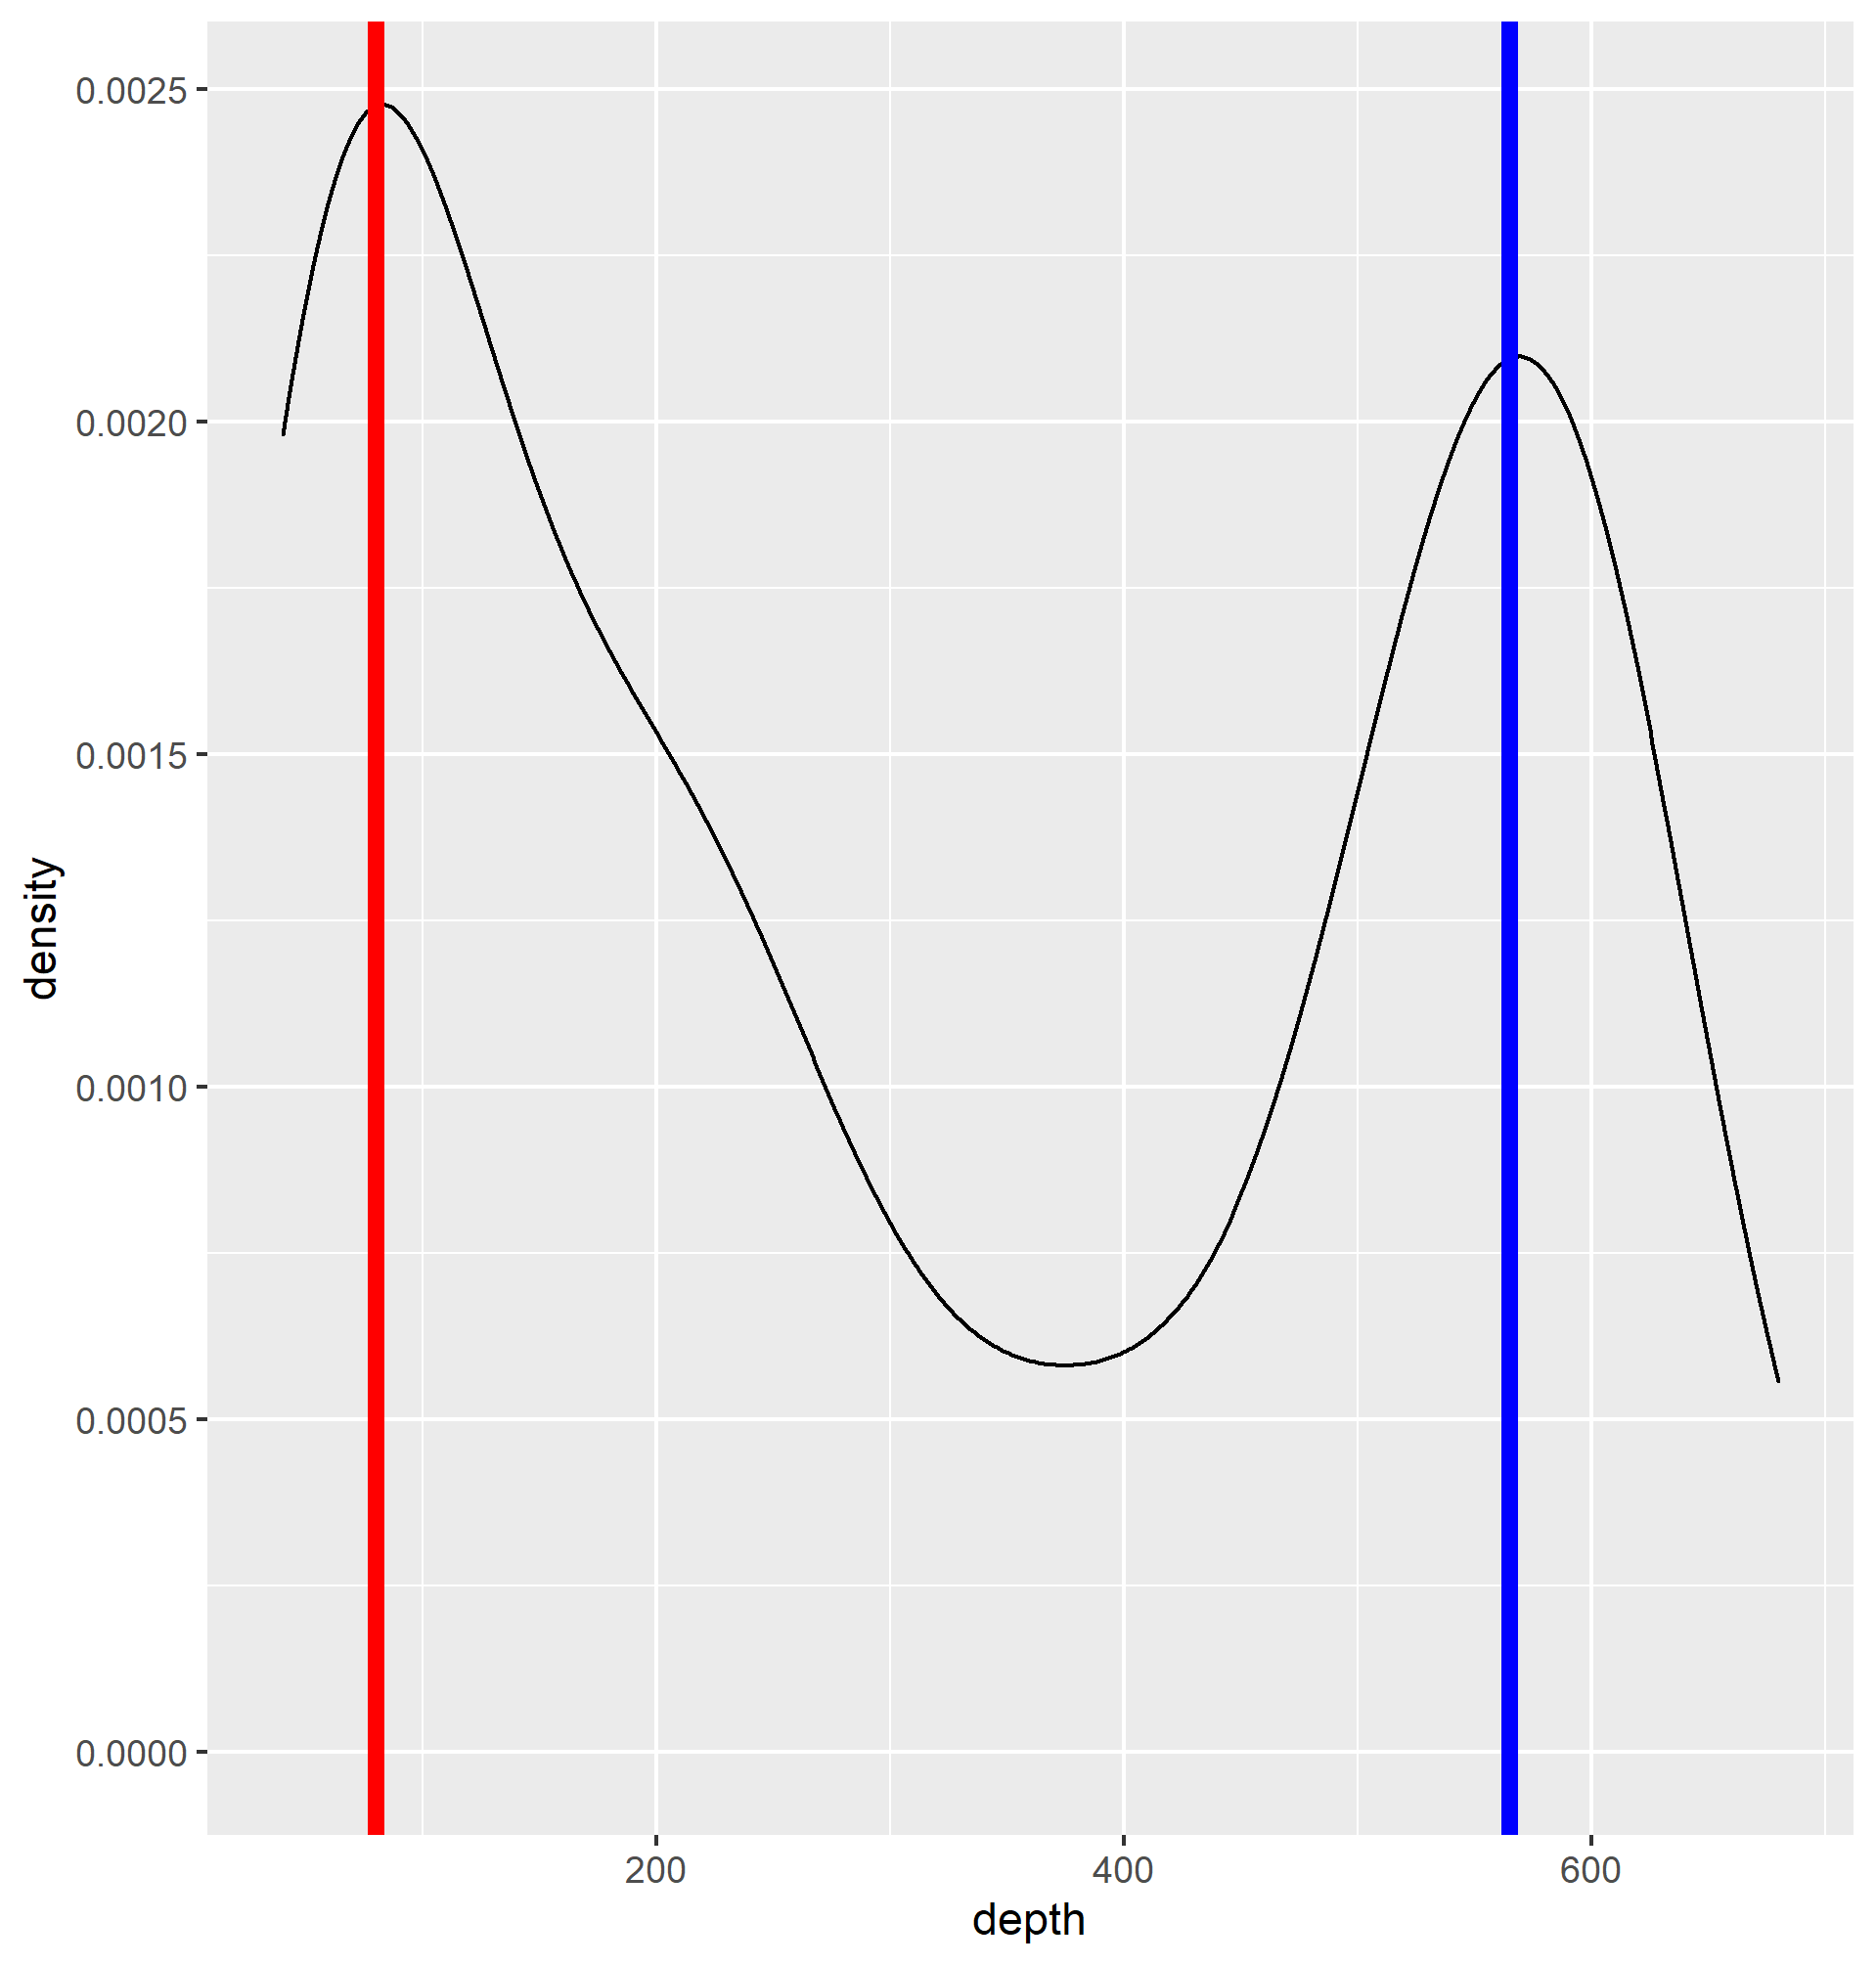
\includegraphics[scale=0.7, keepaspectratio]{ex5/5quakes_depth_dist.png}
\caption{Density plot for  variable \texttt{quakes\$depth}}
\label{5quakes_depth_dist}
\end{figure} 


\begin{figure}[h]
\centering
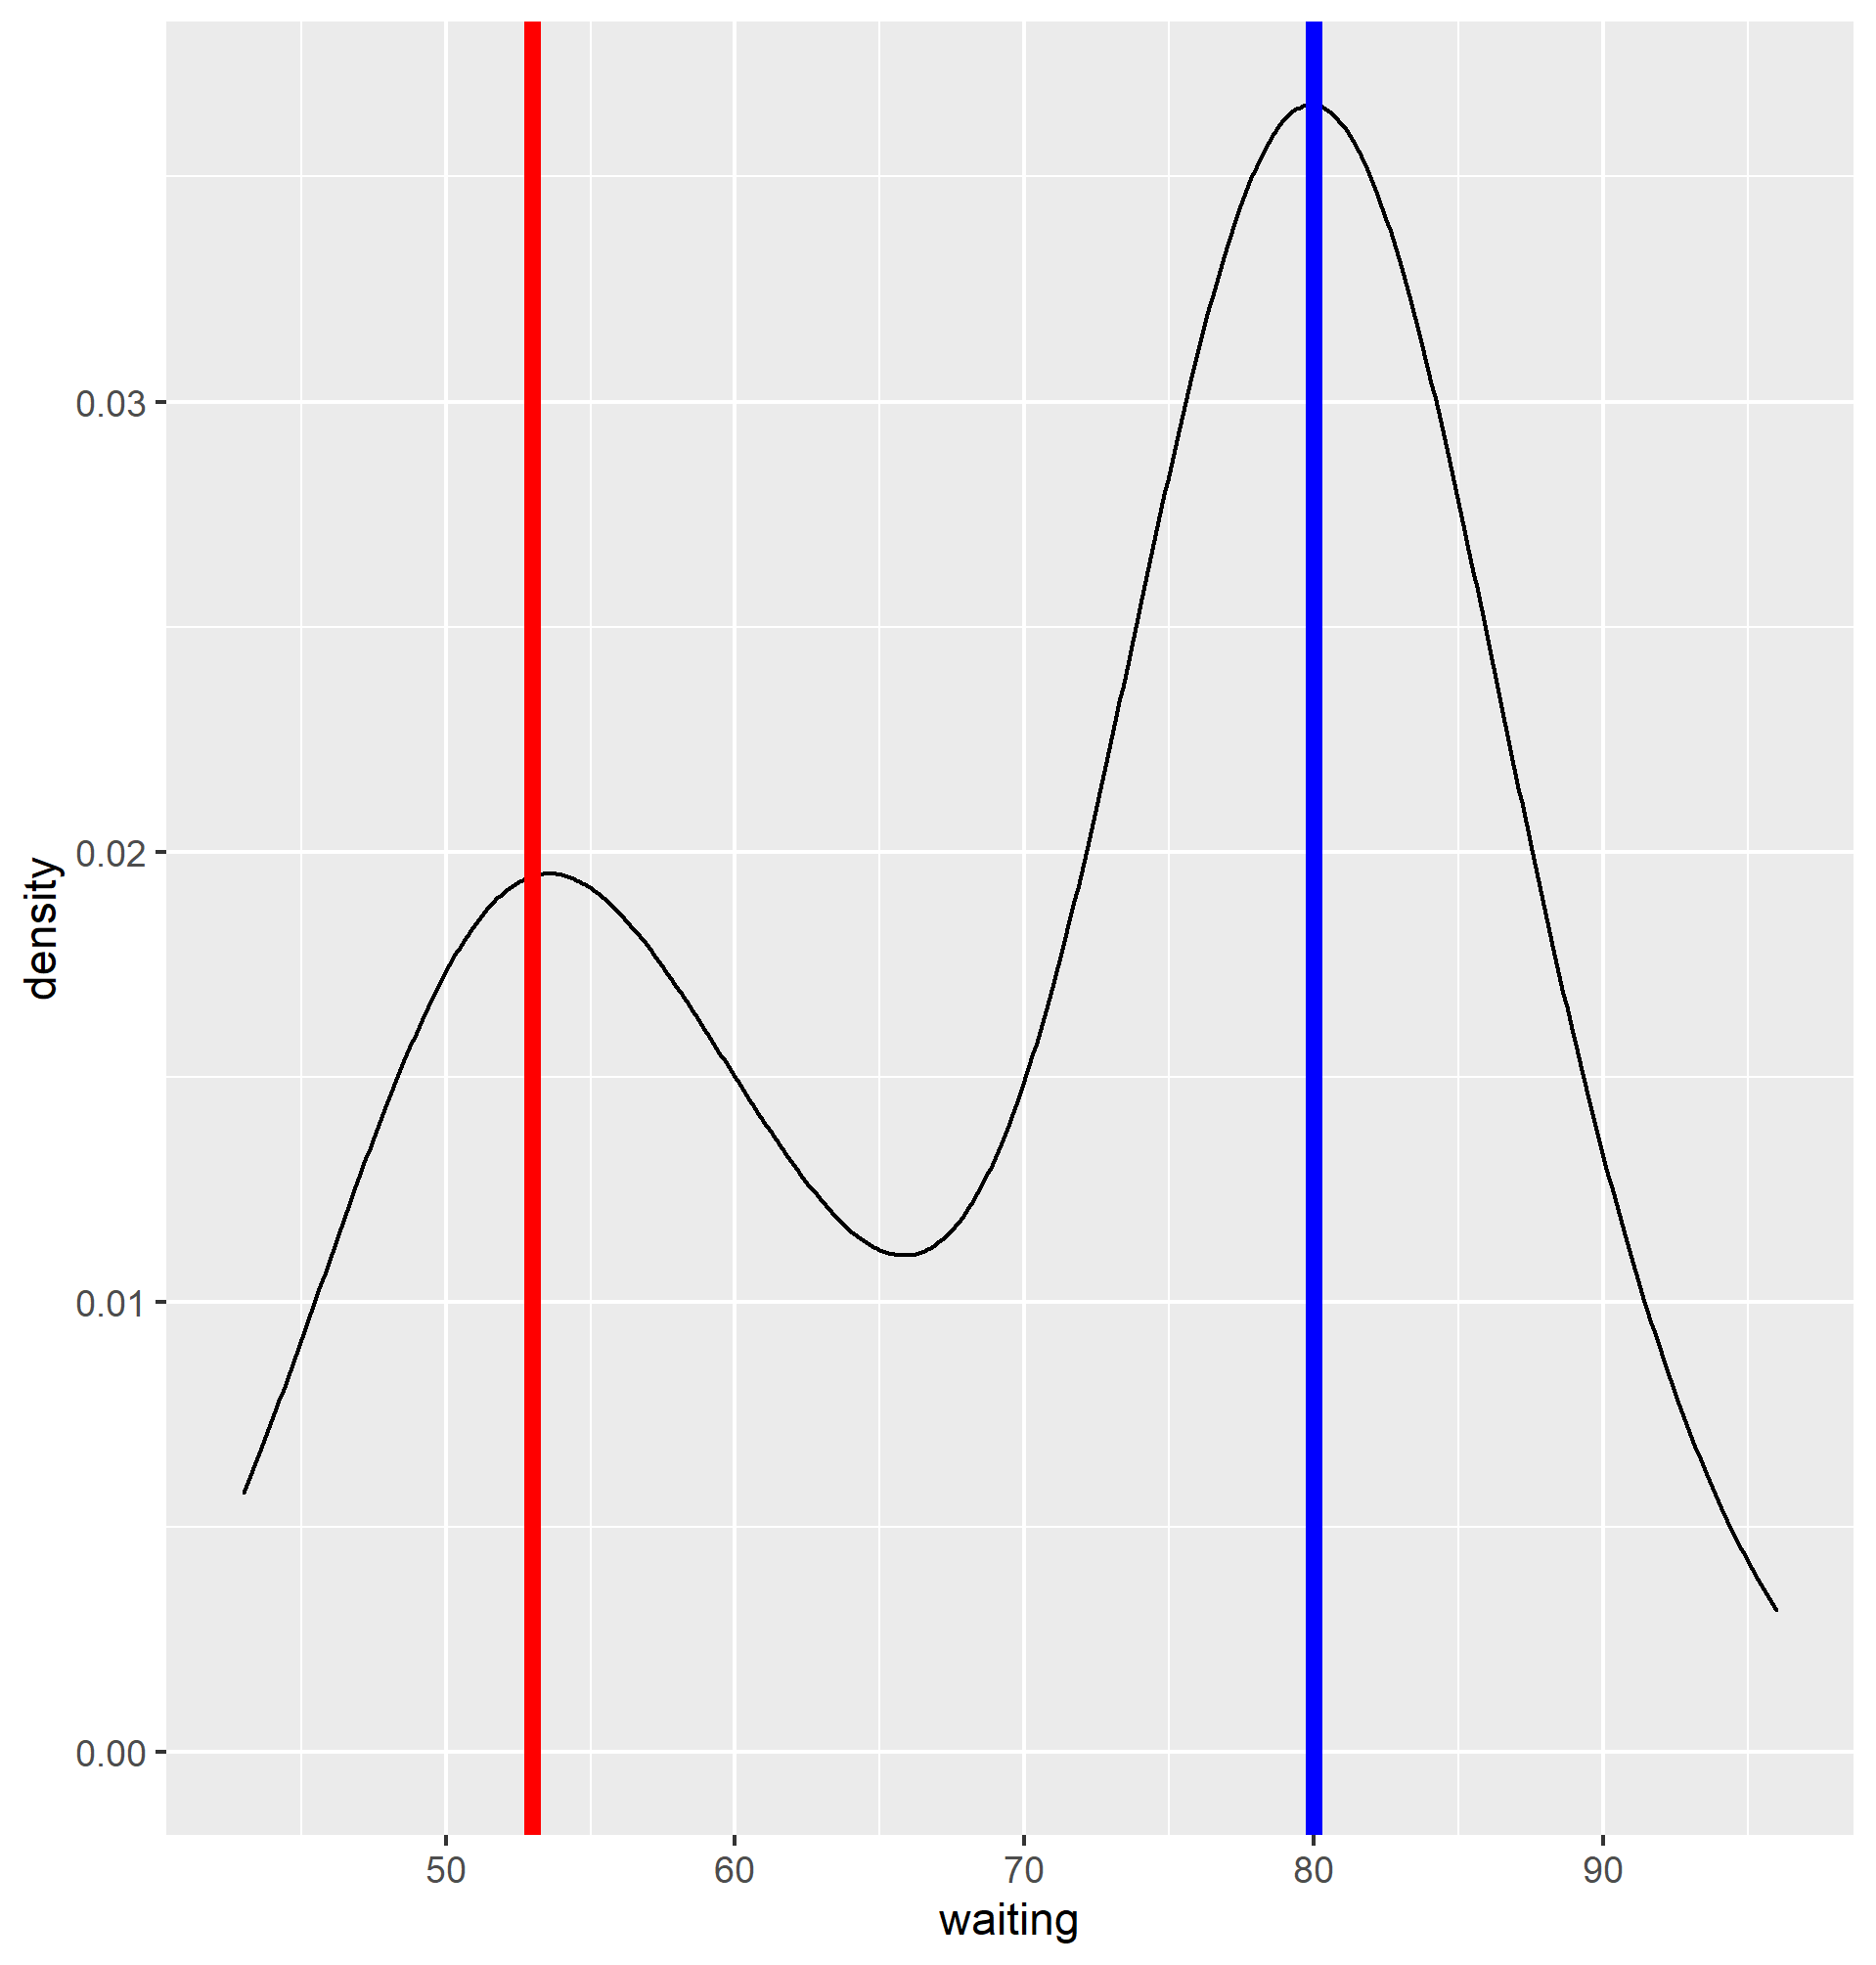
\includegraphics[scale=0.7, keepaspectratio]{ex5/5faith_wait_dist.png}
\caption{Density plot for  variable \texttt{faith\$waiting}}
\label{5faith_wait_dist}
\end{figure}

We can immediately see that the resulting distribution appears to be bi-modal (i.e. there are two bumps in both the plots) suggesting that these in case of both the data, they might be coming from two different sources.


Putting the the \texttt{quakes} data into context suggests that the earthquakes in Fiji may be coming from two different sub-populations, depending upon the depth of the region. Similarly, putting the the \texttt{faithful} data into context suggests that the eruption times may be coming from two different sub-populations. There could be several reasons for this. For instance, maybe at different times of the year the geyser eruptions are more frequent. We can probably take an intuitive guess as to how we could split this data.

For instance, we can observe in Figure \ref{5quakes_depth_dist}, there likely is a sub-population with a mean depth of $\sim 80$ with some variance around this mean (red vertical line in figure \ref{5quakes_depth_dist}.) Another population with a mean depth of $\sim 565$ with again some variance around this mean (blue vertical line in figure \ref{5quakes_depth_dist}). Similarly, as we can observe in Figure \ref{5faith_wait_dist}, there likely is a sub-population with a mean eruption of $\sim 53$ with some variance around this mean (red vertical line in figure \ref{5faith_wait_dist}.) Another population with a mean eruption of $\sim 80$ with again some variance around this mean (blue vertical line in figure \ref{5faith_wait_dist}).

\section{Gaussian Mixture Model}
What we have done is a naive attempt at trying to group the data into sub-populations or clusters.
But surely there must be some objective and “automatic” way of defining these clusters? This is where mixture models come in by providing a “model-based approach” to clustering through the use of statistical distributions.


A mixture model consist of a mixture of distributions. The first thing we need to do when performing mixture model clustering is to determine what type of statistical distribution we want to use for the components.

In our exercise we will use one of the most common statistical distributions used for mixture model clustering which is the Gaussian/Normal Distribution. When Gaussian distributions are used for mixture model clustering, they are referred to as \emph{Gaussian Mixture Models (GMM).} As it turns out, our earlier intuition on where the means and variance of the sub-population in the plot above is a perfect example of how we could apply a GMM. Specifically, we could try to represent each sub-population as its own distribution (aka. mixture component). The entire set of data could then be represented as a mixture of 2 Gaussian distributions (aka. 2-component GMM)

 The procedures is based on the iterative \emph{expectation maximization (EM) algorithm.} The following two points are important to note here. First, the EM algorithm is an iterative procedure, and the time required for it to reach convergence, if it converges at all depends strongly on the problem to which it is applied.  The second key point is that because it is an iterative procedure, the EM algorithm requires starting values for the parameters, and algorithm performance can depend strongly on these initial values.
 
 In our exercise, for both the data sets, we are going take initial values,
 $$\theta^ 0 =(\mu_{1}^{(0)},\mu_{2}^{(0)},\sigma_{1}^{(0)}, \sigma_{2}^{(0)},p^{(0)}) =(m-sd/2, m + sd/2, sd, sd, 0.5)$$
where $m$ is the mean of all observation and $sd$ the standard deviation.

Observe the following plots \ref{5quakes_depth_mix} and \ref{5faith_wait_mix}. We have built a 2-component GMM. So how do we interpret figures \ref{5quakes_depth_mix} and \ref{5faith_wait_mix}? It’s actually quite simply, the red and blue lines simply indicate $2$ different fitted Gaussian distributions.
\begin{figure}[h]
\centering
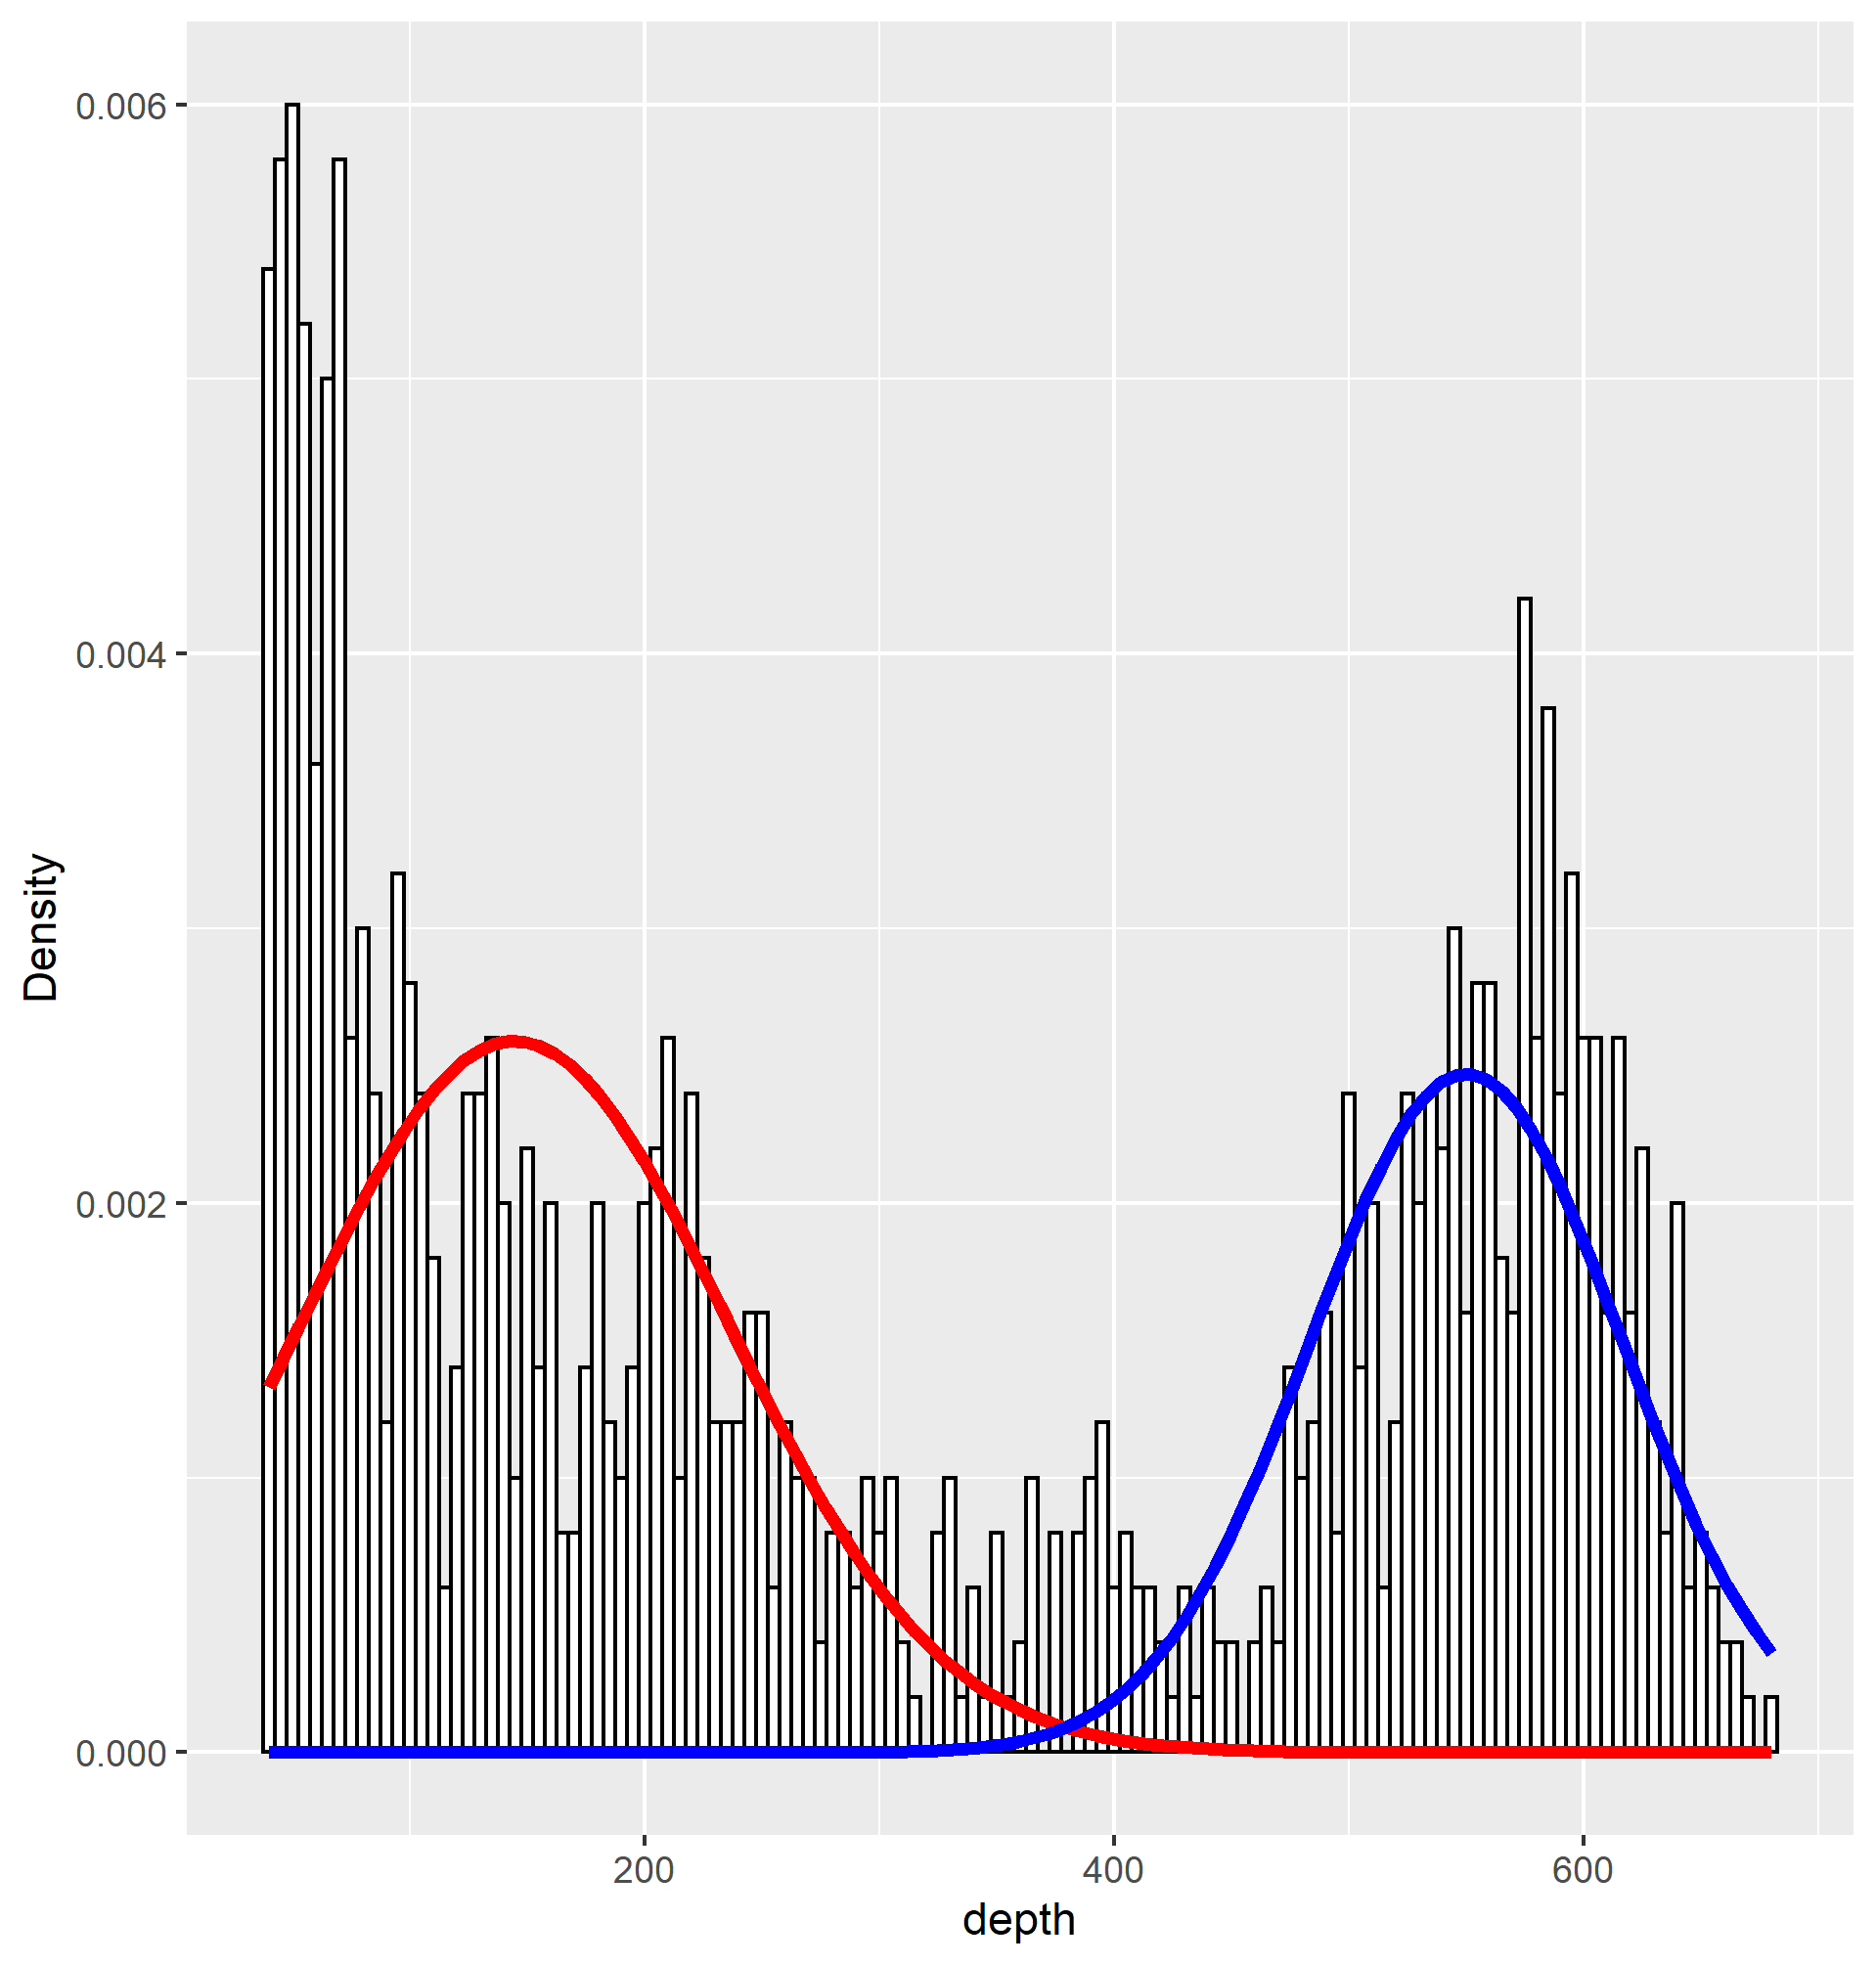
\includegraphics[scale=0.75, keepaspectratio]{ex5/5quakes_depth_mix.png}
\caption{Density plot for  GMM with barplot for \texttt{quakes\$depth}}
\label{5quakes_depth_mix}
\end{figure} 


\begin{figure}[h]
\centering
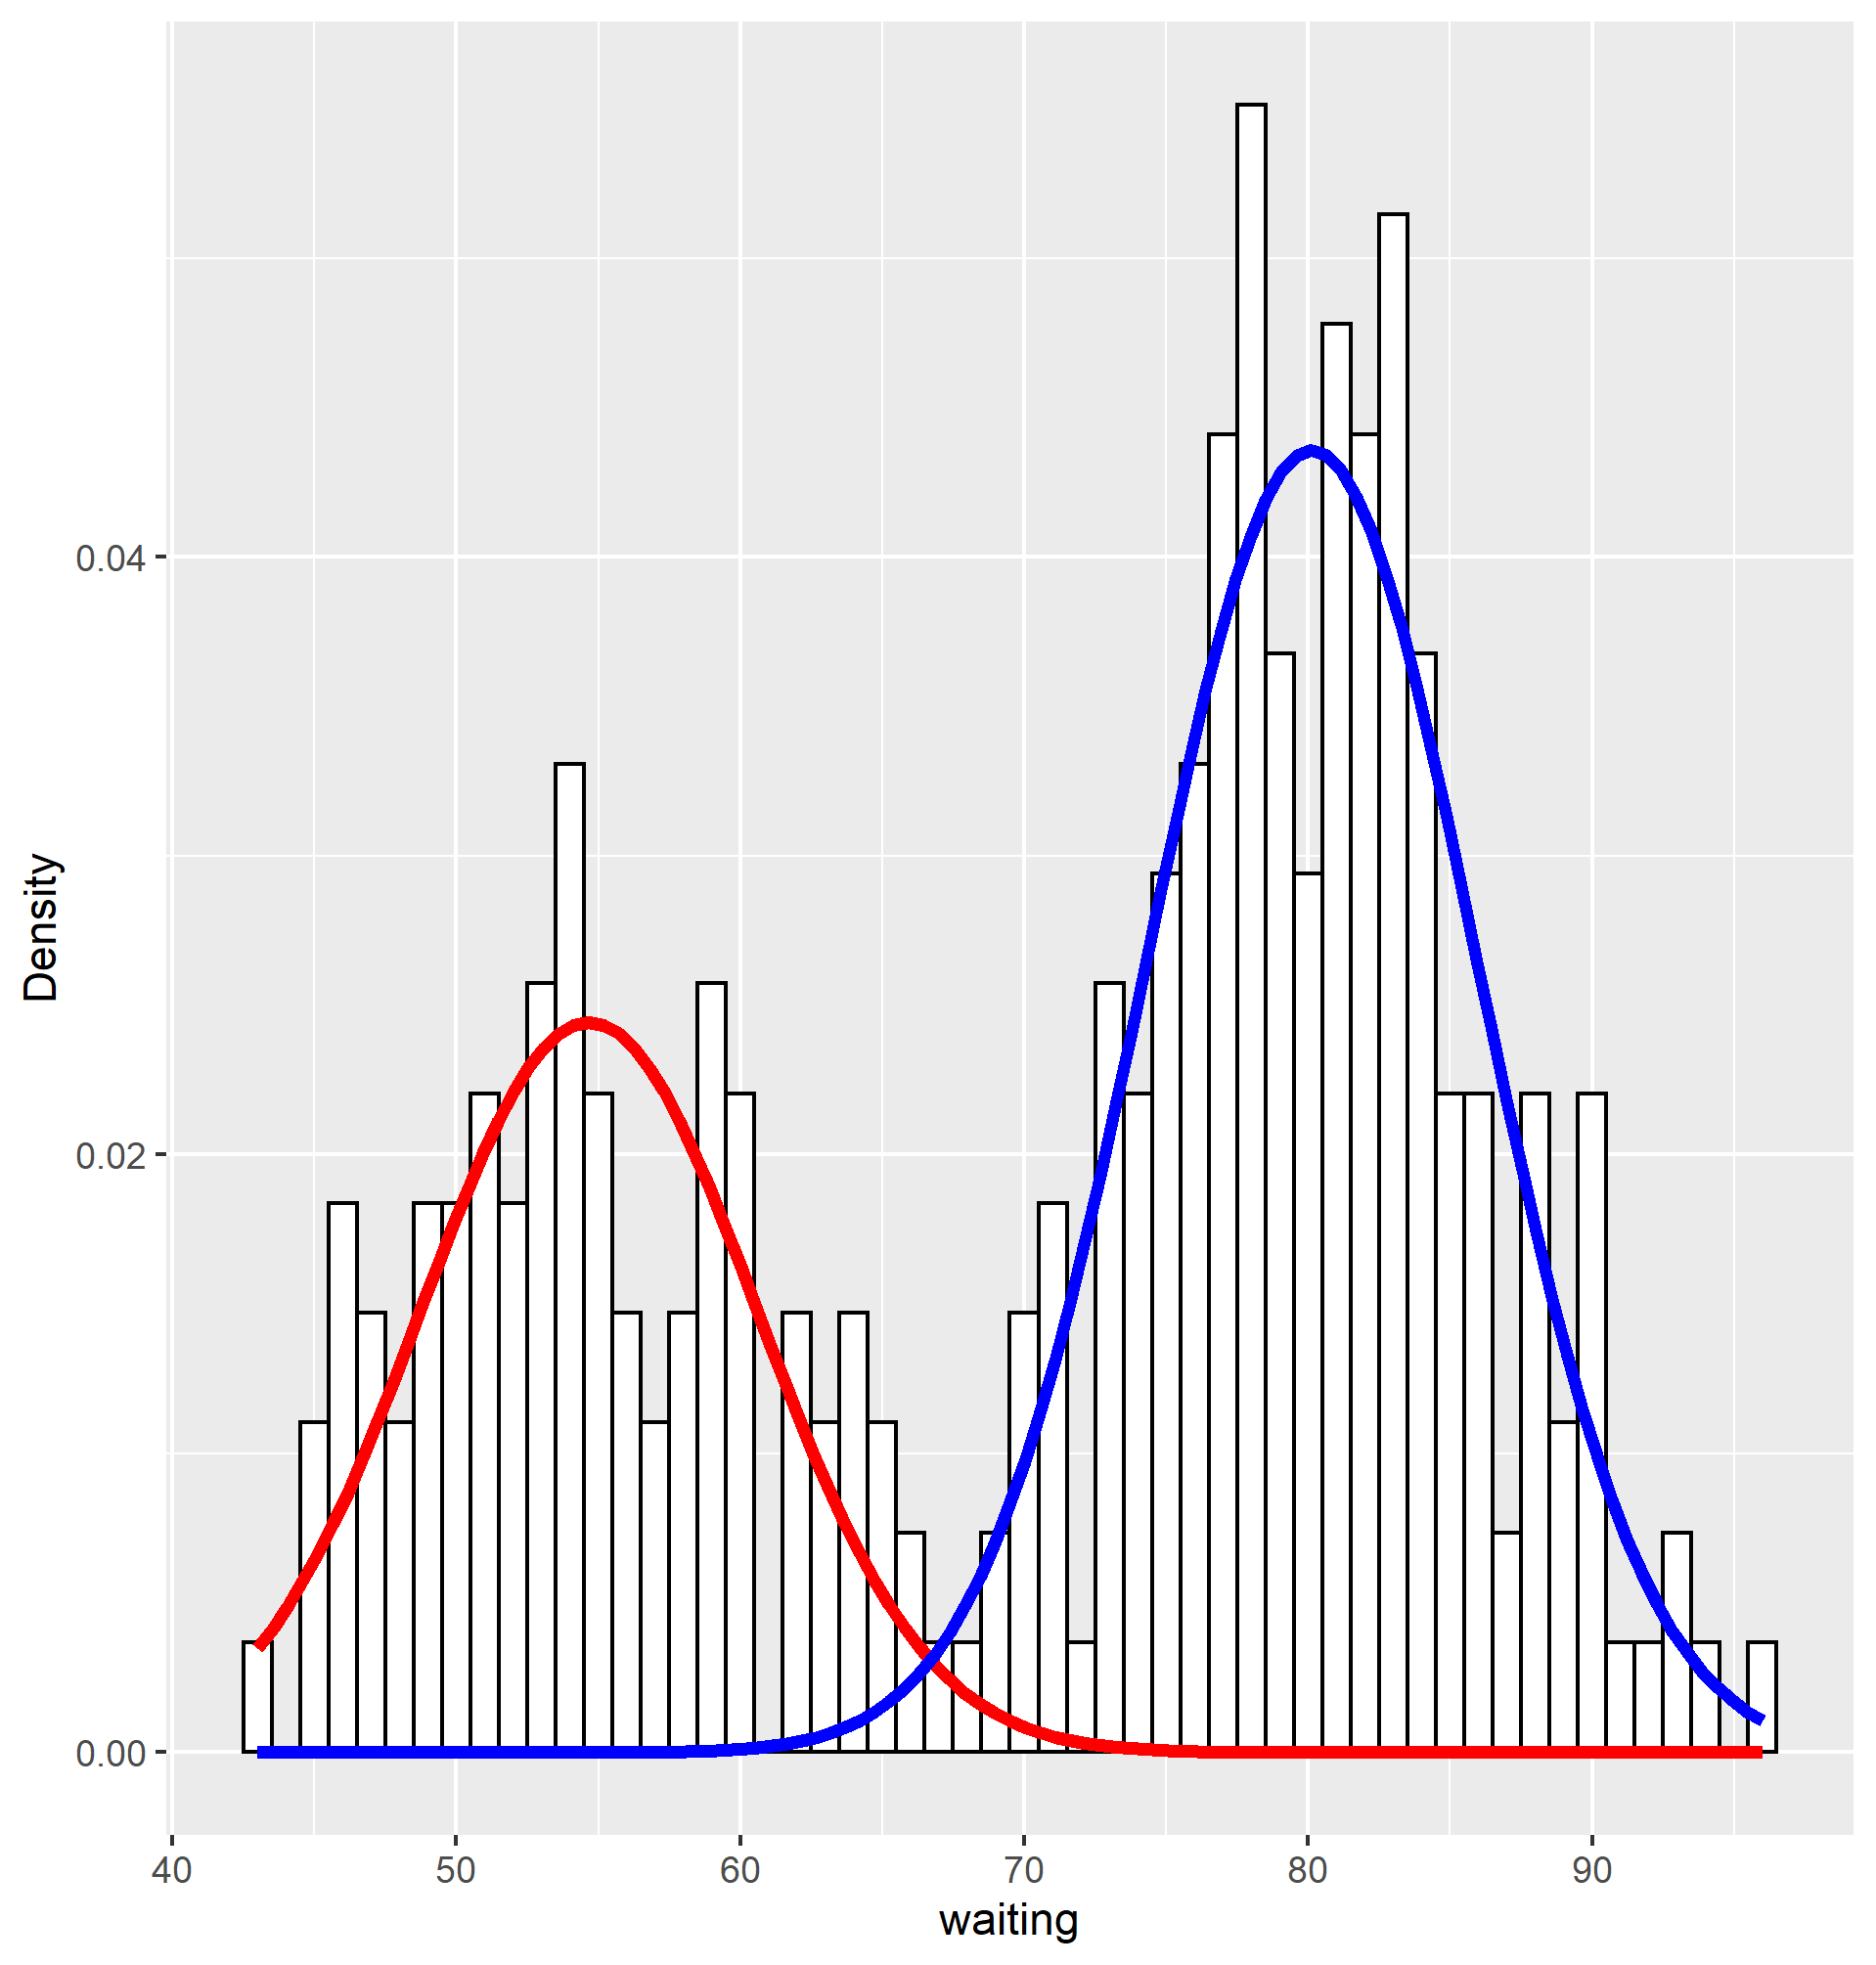
\includegraphics[scale=0.75, keepaspectratio]{ex5/5faith_wait_mix.png}
\caption{Density plot for  GMM with barplot for \texttt{faith\$waiting}}
\label{5faith_wait_mix}
\end{figure}



\section{Stopping criteria}
In the EM-algorithm we have used the (log-)likelihood function, which is a non-decreasing sequence. Also, is strictly increasing unless $\theta^{(k)} = \theta^{(k-1)}.$ We can observe this fact for the two data sets.


\begin{figure}[h]
\centering
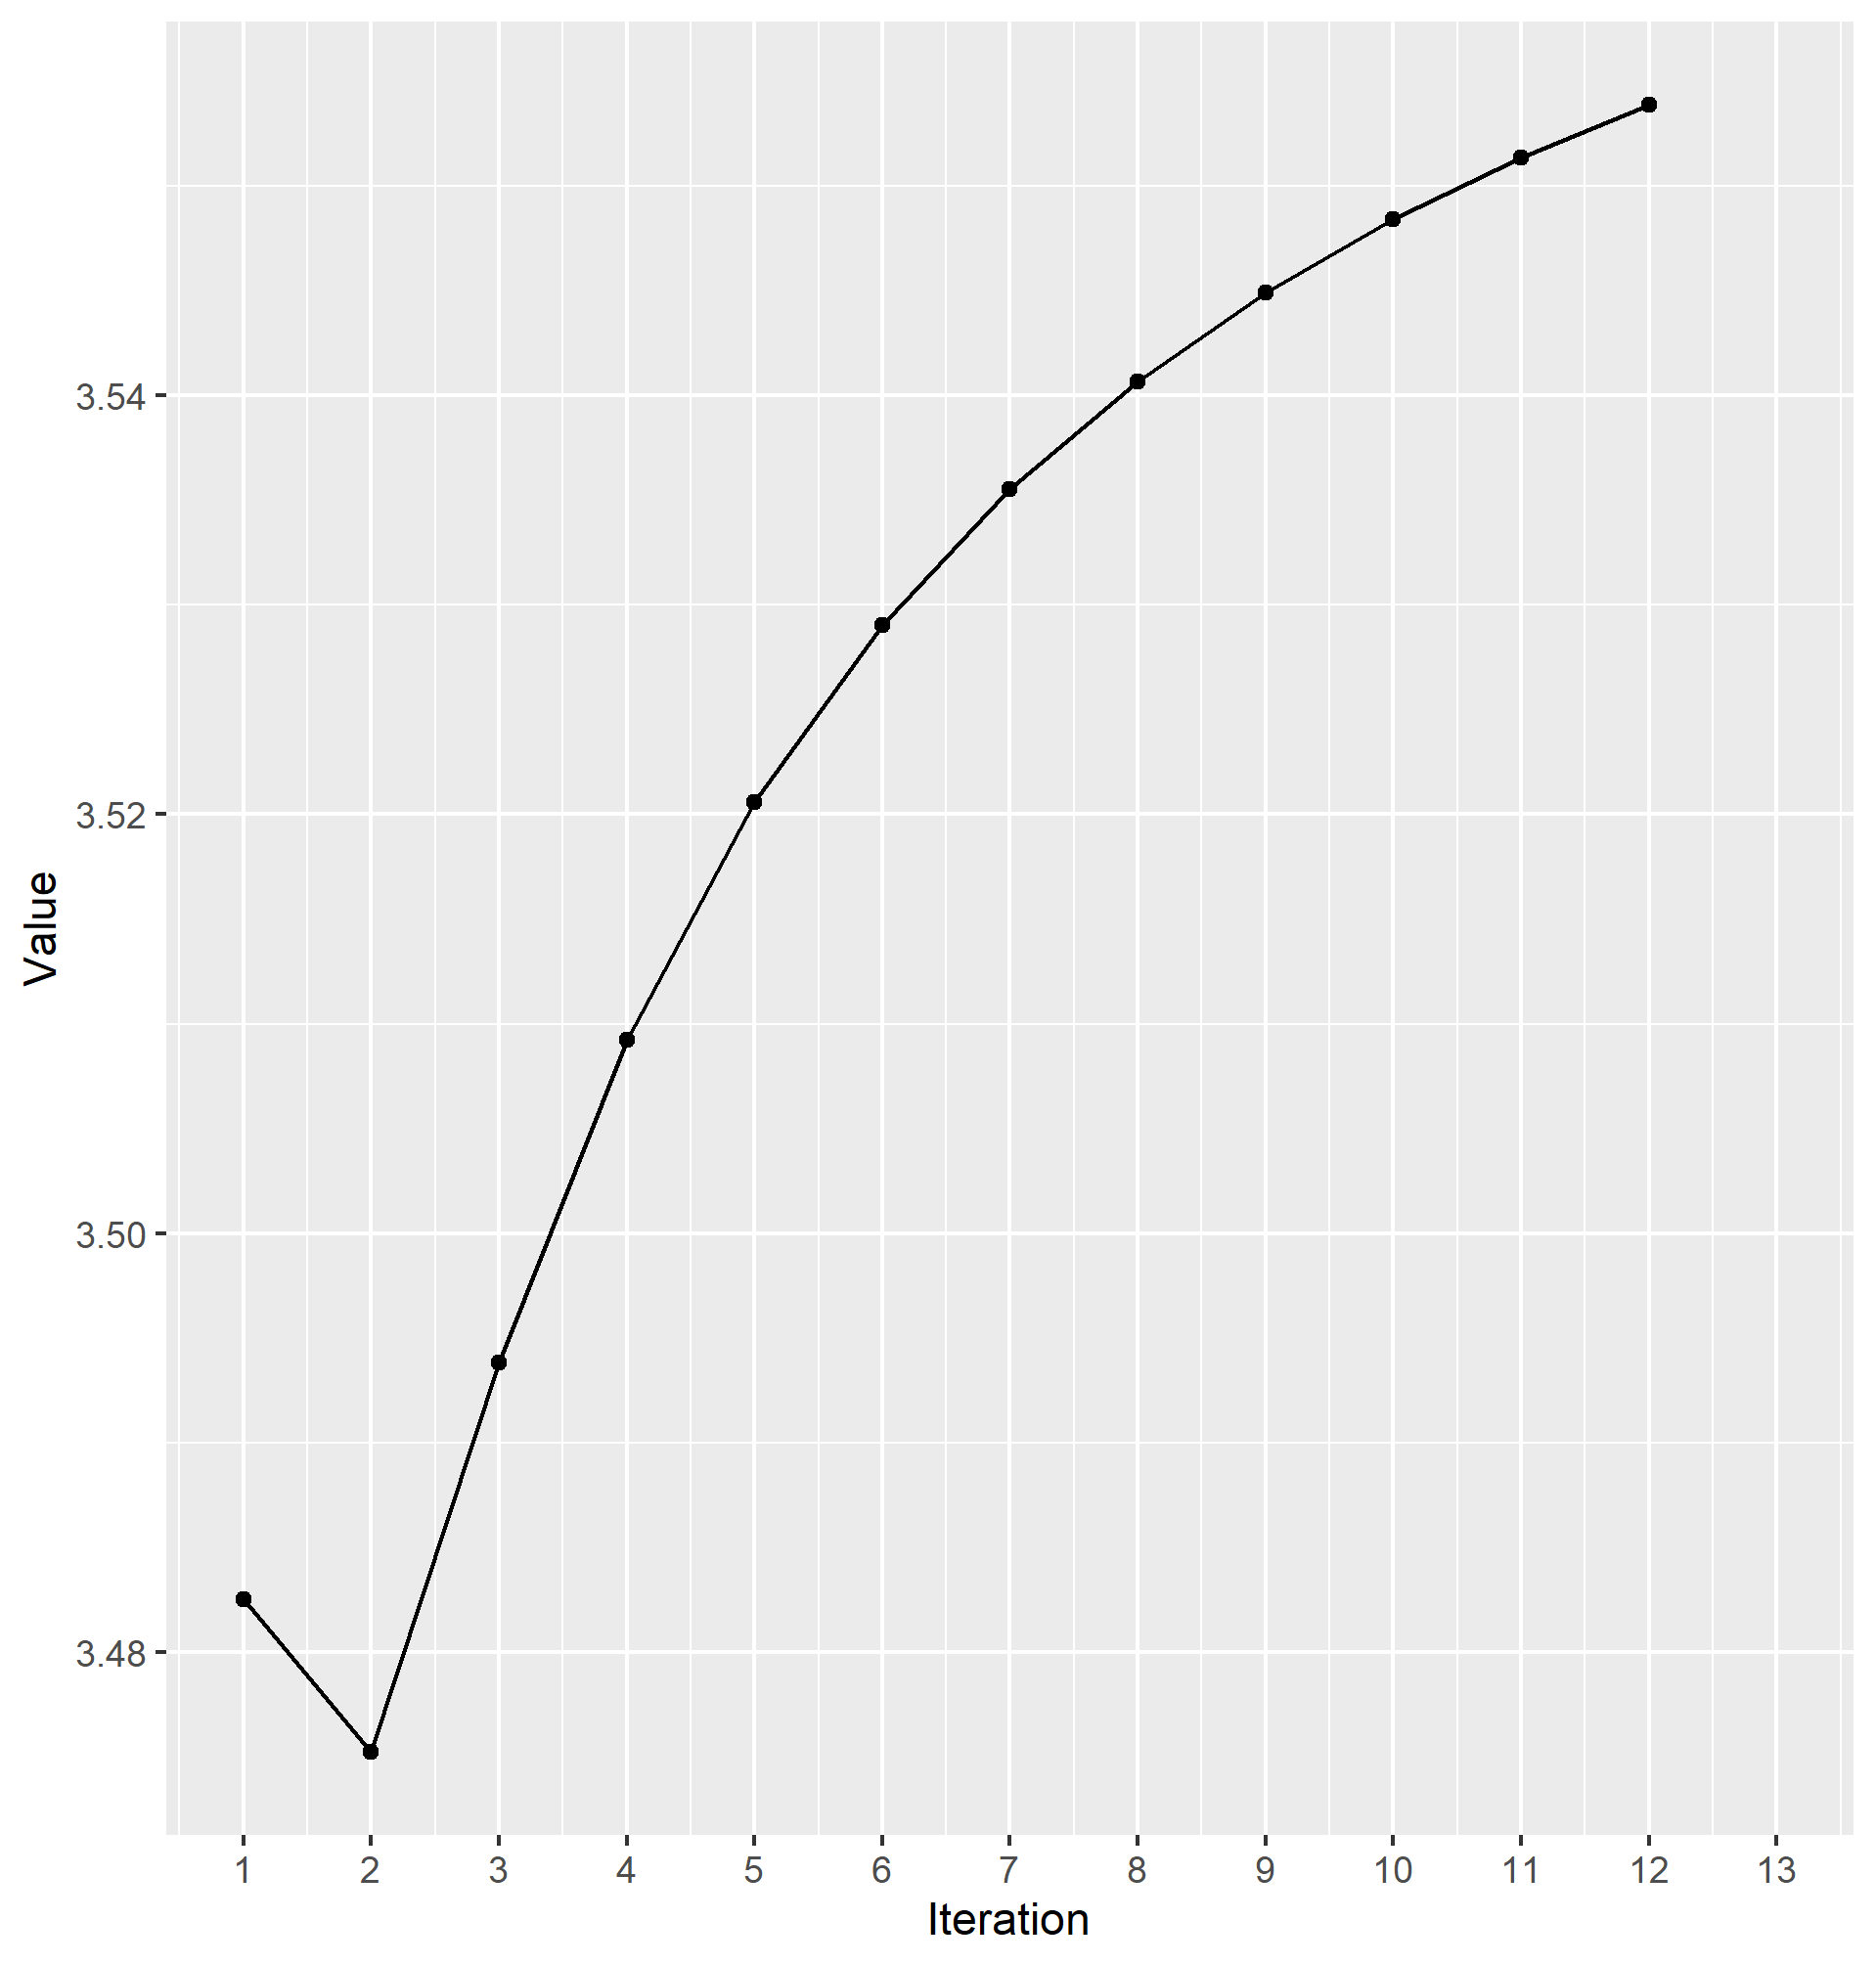
\includegraphics[scale=0.75, keepaspectratio]{ex5/5quakes_depth_iter.png}
\caption{Values of the log-likelihood function per iteration for \texttt{quakes\$depth}}
\label{5quakes_depth_iter}
\end{figure} 


\begin{figure}[h]
\centering
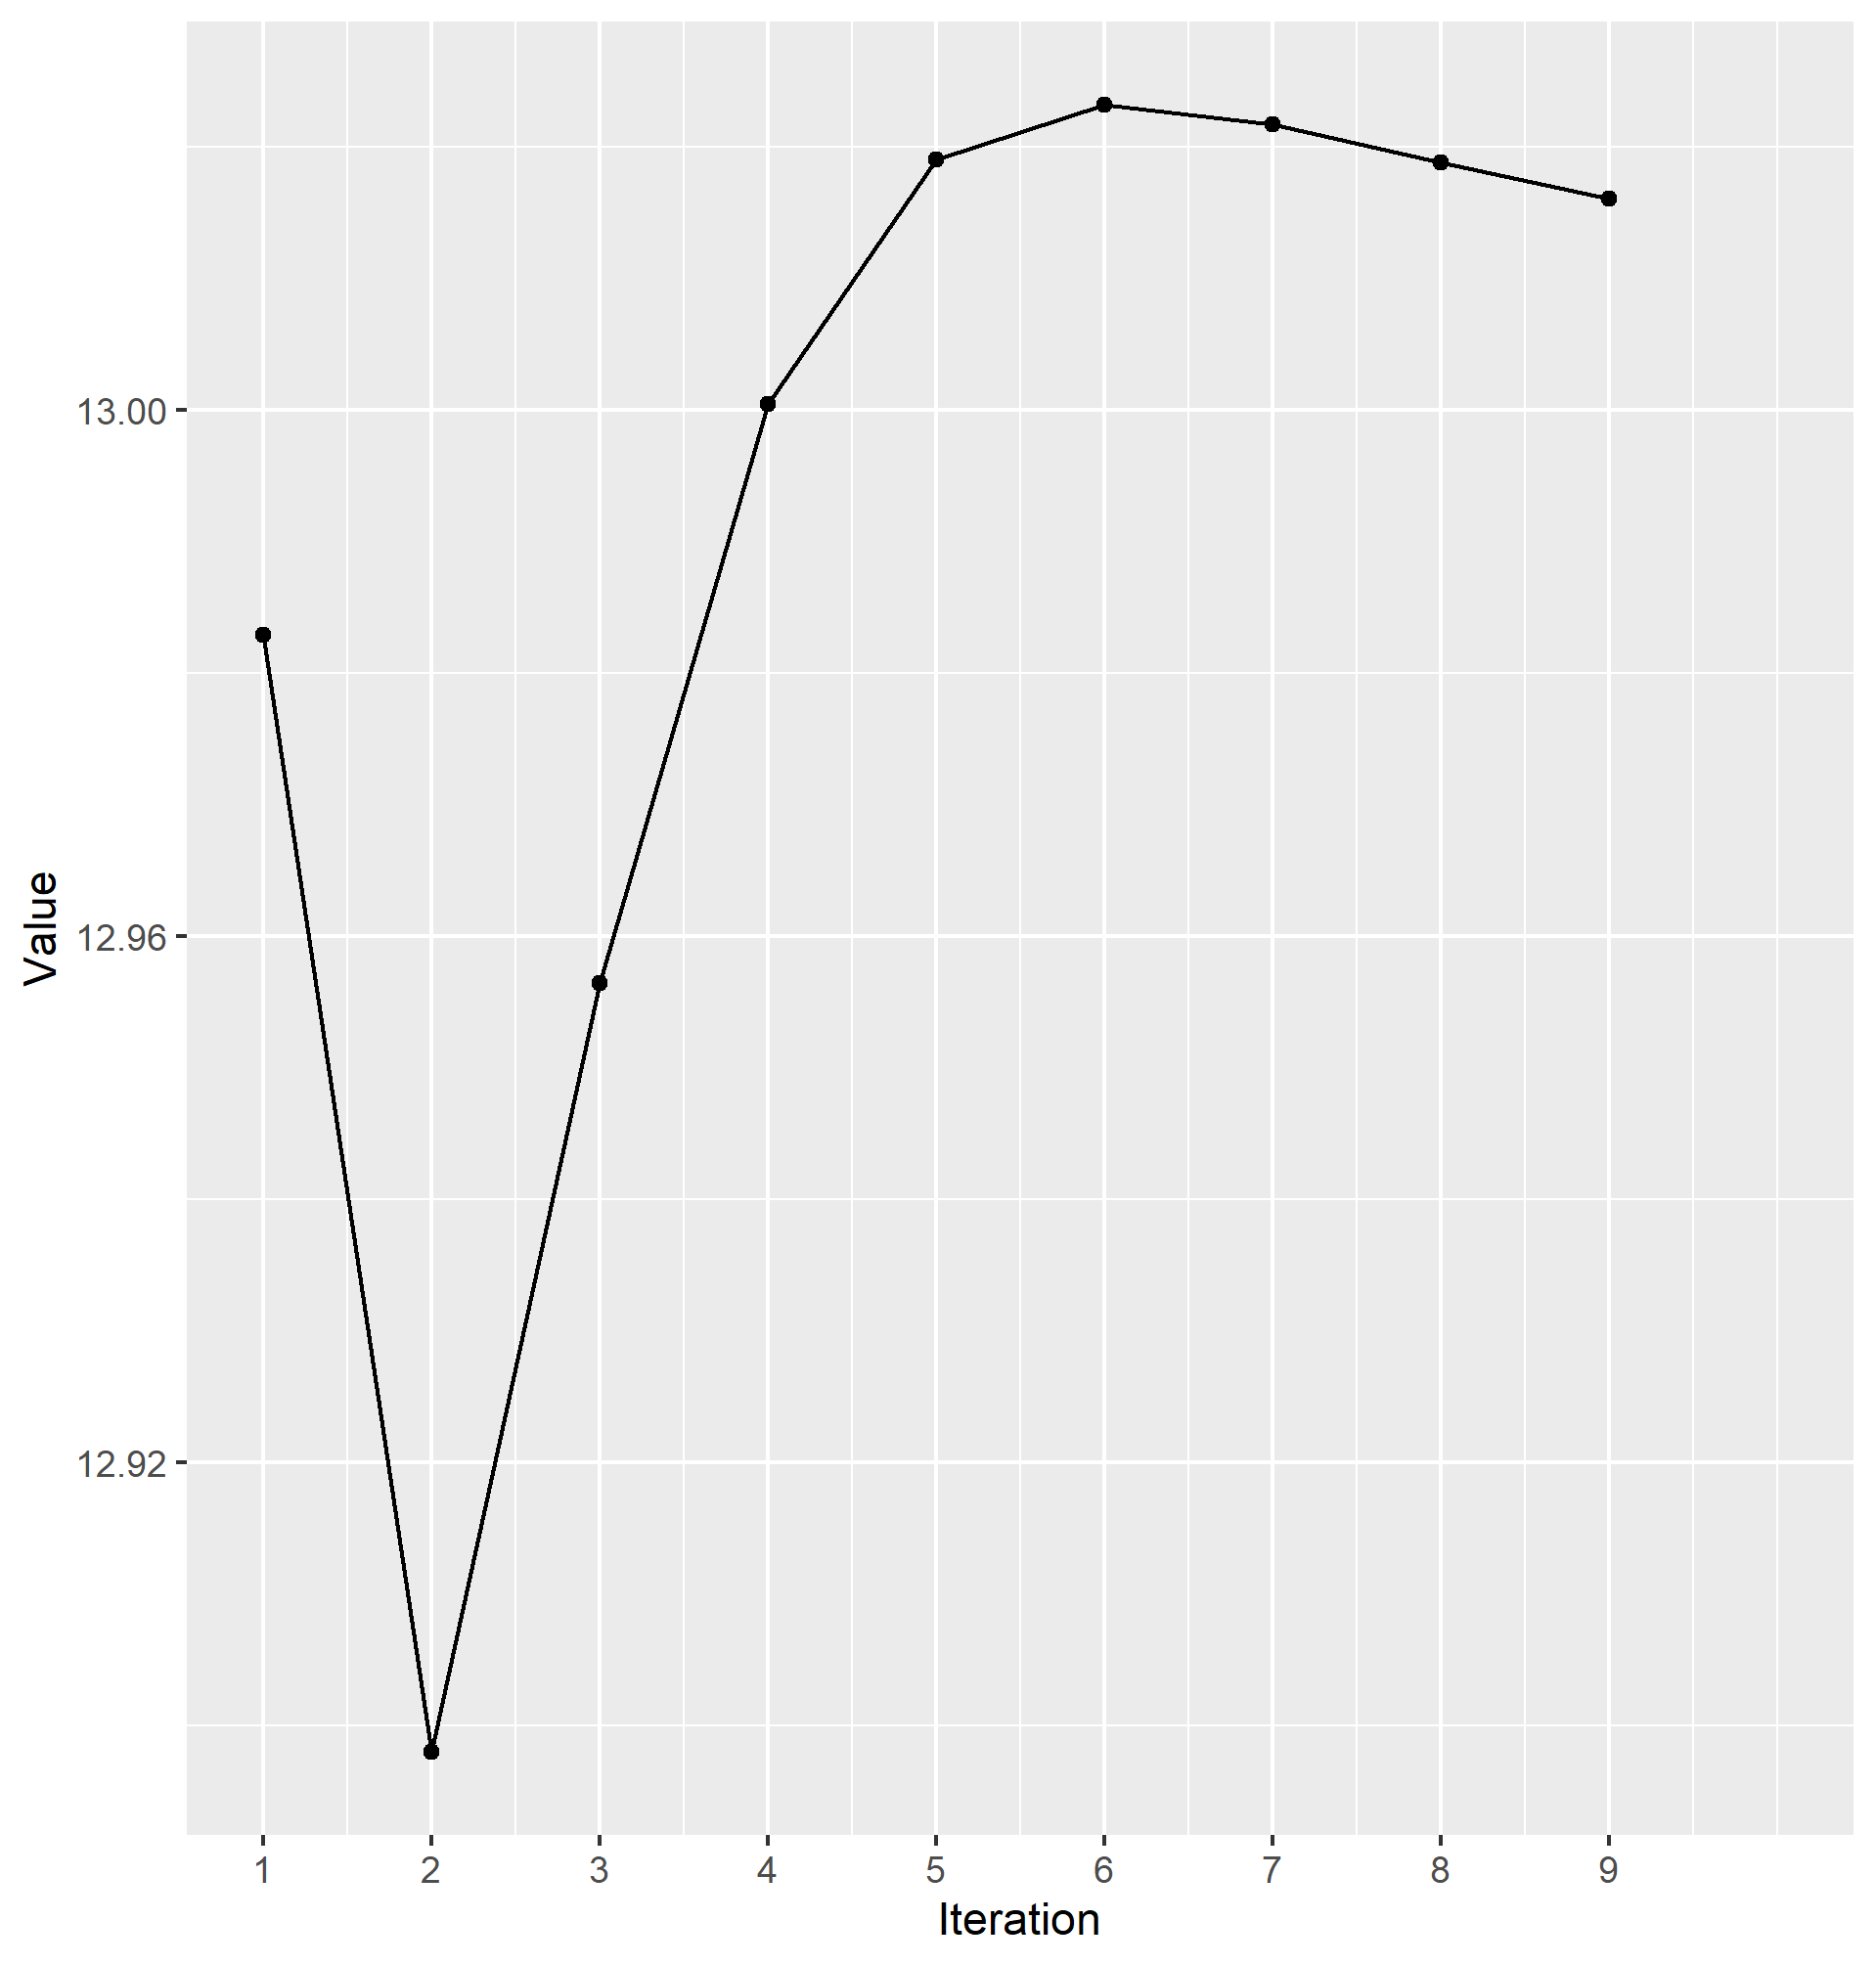
\includegraphics[scale=0.75, keepaspectratio]{ex5/5faith_wait_iter.png}
\caption{Values of the log-likelihood function per iteration for  \texttt{faith\$waiting}}
\label{5faith_wait_iter}
\end{figure}

We can this be used to formulate a stopping criterion for the EM-Algorithm. We can decide a threshold on $\theta^{(k)} - \theta^{(k-1)}$, if it is below the threshold then, we can stop the algorithm. For eg. we have take the threshold as $0.00001$. In the case of \texttt{quakes\$depth} algorithm stopped after $12$ iterations, where as in the case of \texttt{faith\$waiting} it stopped after $9$ iterations.  This just assures that the improvement in the maximization step is small and the algorithm can be stopped.